\section{Lecture 4: Information, Marginalization, and Estimator Design}
\label{sec:lecture04}

\subsection*{Topics}
\begin{itemize}[itemsep=0.3em]
\item the matrix inversion lemma;
\item covariance vs.\ information;
\item marginalization and the Schur complement;
\item why the information matrix reflects problem structure;
\item a typical visual-odometry / SLAM pipeline;
\item many ways to handle $\vect{z}=\vect{h}(\vect{x})+\vect{n}$;
\item designing a common estimator --- deriving the EKF from MAP by marginalization.
\end{itemize}

% Tighten matrix column spacing for the dense block-matrix algebra in this lecture.
\setlength{\arraycolsep}{3.5pt}

% =====================================================================
\subsection{The matrix inversion lemma}

For a $2\times2$ block matrix, the inverse can be written block by block. In the general form,
\begin{align}
\begin{bmatrix} \vect{A} & \vect{B} \\ \vect{C} & \vect{D} \end{bmatrix}^{-1}
= \begin{bmatrix} \vect{E} & \vect{F} \\ \vect{G} & \vect{H} \end{bmatrix}, \qquad
\begin{cases}
\vect{E} = (\vect{A} - \vect{B}\vect{D}^{-1}\vect{C})^{-1}, \\[2pt]
\vect{F} = -\vect{E}\vect{B}\vect{D}^{-1}, \\[2pt]
\vect{G} = -\vect{D}^{-1}\vect{C}\vect{E}, \\[2pt]
\vect{H} = \vect{D}^{-1} + \vect{D}^{-1}\vect{C}\vect{E}\vect{B}\vect{D}^{-1}.
\end{cases}
\end{align}
For the symmetric case ($\vect{C}=\vect{B}\trans$, so the inverse is symmetric too),
\begin{align}
\begin{bmatrix} \vect{A} & \vect{B} \\ \vect{B}\trans & \vect{D} \end{bmatrix}^{-1}
= \begin{bmatrix} \vect{E} & \vect{F} \\ \vect{F}\trans & \vect{H} \end{bmatrix}, \qquad
\begin{aligned}
\vect{E} &= (\vect{A} - \vect{B}\vect{D}^{-1}\vect{B}\trans)^{-1}, \\
\vect{F} &= -\vect{E}\vect{B}\vect{D}^{-1}, \\
\vect{H} &= \vect{D}^{-1} + \vect{D}^{-1}\vect{B}\trans\vect{E}\vect{B}\vect{D}^{-1} = (\vect{D} - \vect{B}\trans\vect{A}^{-1}\vect{B})^{-1}.
\end{aligned}
\end{align}
The term $\vect{A} - \vect{B}\vect{D}^{-1}\vect{B}\trans$ (resp.\ $\vect{D} - \vect{B}\trans\vect{A}^{-1}\vect{B}$) is the \emph{Schur complement}. This is one of the most important matrix operations for the derivations that follow.

% =====================================================================
\subsection{Covariance and information}

Recall the measurement model from Lecture~1, $\vect{z} = \vect{h}(\vect{x}) + \vect{n}$ with $\vect{n}\sim\mathcal{N}(\vect{0},\vect{R})$ and $\vect{R}$ the noise covariance. The MAP / weighted-least-squares estimate is
\begin{align}
\max_{\vect{x}} \; p(\vect{z}\mid\vect{x}) \;\Leftrightarrow\; \min_{\vect{x}} \; \norm{\vect{z} - \vect{h}(\vect{x})}_{\vect{R}}^{2}.
\end{align}
Given a linearization point $\hat{\vect{x}}$, $\vect{z} = \vect{h}(\hat{\vect{x}}) + \vect{H}\tilde{\vect{x}} + \vect{n}$, so with the residual $\tilde{\vect{z}} = \vect{z} - \vect{h}(\hat{\vect{x}})$,
\begin{align}
\tilde{\vect{z}} = \vect{H}\tilde{\vect{x}} + \vect{n}.
\end{align}
The normal equations and their solution are
\begin{empheq}[box=\fbox]{align}
\underbrace{\vect{H}\trans\vect{R}^{-1}\vect{H}}_{\text{information}}\,\tilde{\vect{x}} = \vect{H}\trans\vect{R}^{-1}\tilde{\vect{z}}, \qquad
\tilde{\vect{x}} = \big(\vect{H}\trans\vect{R}^{-1}\vect{H}\big)^{-1}\vect{H}\trans\vect{R}^{-1}\tilde{\vect{z}}.
\end{empheq}
To find the covariance of the corrected estimate $\vect{x}^{\oplus} = \hat{\vect{x}} + \tilde{\vect{x}}$, substitute $\tilde{\vect{z}} = \vect{H}(\vect{x}-\hat{\vect{x}}) + \vect{n}$:
\begin{align}
\vect{x}^{\oplus}
&= \hat{\vect{x}} + \big(\vect{H}\trans\vect{R}^{-1}\vect{H}\big)^{-1}\vect{H}\trans\vect{R}^{-1}\tilde{\vect{z}} \\
&= \hat{\vect{x}} + \big(\vect{H}\trans\vect{R}^{-1}\vect{H}\big)^{-1}\vect{H}\trans\vect{R}^{-1}\big(\vect{H}(\vect{x}-\hat{\vect{x}}) + \vect{n}\big) \\
&= \vect{x} + \big(\vect{H}\trans\vect{R}^{-1}\vect{H}\big)^{-1}\vect{H}\trans\vect{R}^{-1}\vect{n}.
\end{align}
Hence $\vect{x} - \vect{x}^{\oplus} = -(\vect{H}\trans\vect{R}^{-1}\vect{H})^{-1}\vect{H}\trans\vect{R}^{-1}\vect{n}$, and
\begin{align}
\vect{P}_{\vect{x}^{\oplus}\vect{x}^{\oplus}}
&= \E\big[(\vect{x}-\vect{x}^{\oplus})(\vect{x}-\vect{x}^{\oplus})\trans\big] \notag \\
&= \big(\vect{H}\trans\vect{R}^{-1}\vect{H}\big)^{-1}\vect{H}\trans\vect{R}^{-1}\,\E(\vect{n}\vect{n}\trans)\,\vect{R}^{-1}\vect{H}\big(\vect{H}\trans\vect{R}^{-1}\vect{H}\big)^{-1} \\
&= \big(\vect{H}\trans\vect{R}^{-1}\vect{H}\big)^{-1},
\end{align}
using $\E(\vect{n}\vect{n}\trans) = \vect{R}$. Therefore information and covariance are inverses of each other:
\begin{empheq}[box=\fbox]{align}
\text{information}\quad \vect{\Sigma} = \vect{H}\trans\vect{R}^{-1}\vect{H}, \qquad
\text{covariance}\quad \vect{P} = \big(\vect{H}\trans\vect{R}^{-1}\vect{H}\big)^{-1}, \qquad
\vect{\Sigma} = \vect{P}^{-1}, \;\; \vect{P} = \vect{\Sigma}^{-1}.
\end{empheq}
This is fundamental for what follows:
\begin{itemize}[noitemsep,topsep=2pt]
\item for \textbf{optimization / least squares}, we keep track of the information matrix $\vect{\Sigma}$;
\item for \textbf{filtering (EKF)}, we keep track of the covariance $\vect{P}$.
\end{itemize}

% =====================================================================
\subsection{Marginalization}

Let $\vect{x}\sim\mathcal{N}(\hat{\vect{x}},\vect{P}_{\vect{xx}})$, where $\hat{\vect{x}}$ is the best estimate and $\vect{P}_{\vect{xx}}$ the covariance. Partition the state as $\vect{x} = [\vect{x}_A\trans,\vect{x}_B\trans]\trans$, with $\vect{x}_A$ and $\vect{x}_B$ both part of $\vect{x}$:
\begin{align}
\vect{x} \sim \mathcal{N}\!\left(\begin{bmatrix} \hat{\vect{x}}_A \\ \hat{\vect{x}}_B \end{bmatrix},\;
\begin{bmatrix} \vect{P}_{AA} & \vect{P}_{AB} \\ \vect{P}_{BA} & \vect{P}_{BB} \end{bmatrix}\right), \qquad
\vect{P}\trans = \vect{P} \;\text{(SPD)}, \quad \vect{P}_{AB} = \vect{P}_{BA}\trans.
\end{align}
\paragraph{Covariance form (easy).} The marginal of either block is read off directly:
\begin{align}
\vect{x}_A \sim \mathcal{N}(\hat{\vect{x}}_A,\vect{P}_{AA}), \qquad
\vect{x}_B \sim \mathcal{N}(\hat{\vect{x}}_B,\vect{P}_{BB}).
\end{align}
Marginalization in covariance form is straightforward: just keep the corresponding diagonal block.

\paragraph{Information form (Schur complement).} For optimization we work with the information system $(\vect{H}\trans\vect{R}^{-1}\vect{H})\tilde{\vect{x}} = \vect{H}\trans\vect{R}^{-1}\tilde{\vect{z}}$, i.e.
\begin{align}
\vect{\Sigma}\,\tilde{\vect{x}} = \vect{b}, \qquad
\begin{bmatrix} \vect{\Sigma}_{AA} & \vect{\Sigma}_{AB} \\ \vect{\Sigma}_{AB}\trans & \vect{\Sigma}_{BB} \end{bmatrix}
\begin{bmatrix} \tilde{\vect{x}}_A \\ \tilde{\vect{x}}_B \end{bmatrix}
= \begin{bmatrix} \vect{b}_A \\ \vect{b}_B \end{bmatrix},
\end{align}
where $\vect{\Sigma}$ is the information matrix and $\vect{b}$ the residual vector. We seek $\vect{\Sigma}_{AA}',\vect{b}_A'$ (and $\vect{\Sigma}_{BB}',\vect{b}_B'$) such that $\vect{\Sigma}_{AA}'\tilde{\vect{x}}_A = \vect{b}_A'$ and $\vect{\Sigma}_{BB}'\tilde{\vect{x}}_B = \vect{b}_B'$ hold after eliminating the other block.

Solving $\vect{\Sigma}\tilde{\vect{x}} = \vect{b}$ via the block inverse,
\begin{align}
\begin{bmatrix} \tilde{\vect{x}}_A \\ \tilde{\vect{x}}_B \end{bmatrix}
= \begin{bmatrix} \vect{\Sigma}_{AA} & \vect{\Sigma}_{AB} \\ \vect{\Sigma}_{AB}\trans & \vect{\Sigma}_{BB} \end{bmatrix}^{-1}
\begin{bmatrix} \vect{b}_A \\ \vect{b}_B \end{bmatrix}
= \begin{bmatrix} \vect{P}_{AA} & \vect{P}_{AB} \\ \vect{P}_{AB}\trans & \vect{P}_{BB} \end{bmatrix}
\begin{bmatrix} \vect{b}_A \\ \vect{b}_B \end{bmatrix}
= \begin{bmatrix} \vect{P}_{AA}\vect{b}_A + \vect{P}_{AB}\vect{b}_B \\ \vect{P}_{AB}\trans\vect{b}_A + \vect{P}_{BB}\vect{b}_B \end{bmatrix},
\end{align}
with the blocks of the inverse given by the matrix inversion lemma,
\begin{align}
\vect{P}_{AA} &= \big(\vect{\Sigma}_{AA} - \vect{\Sigma}_{AB}\vect{\Sigma}_{BB}^{-1}\vect{\Sigma}_{AB}\trans\big)^{-1}, \qquad
\vect{P}_{AB} = -\vect{P}_{AA}\vect{\Sigma}_{AB}\vect{\Sigma}_{BB}^{-1}, \\
\vect{P}_{BB} &= \vect{\Sigma}_{BB}^{-1} + \vect{\Sigma}_{BB}^{-1}\vect{\Sigma}_{AB}\trans\vect{P}_{AA}\vect{\Sigma}_{AB}\vect{\Sigma}_{BB}^{-1}
= \big(\vect{\Sigma}_{BB} - \vect{\Sigma}_{AB}\trans\vect{\Sigma}_{AA}^{-1}\vect{\Sigma}_{AB}\big)^{-1}.
\end{align}
For the $A$ block,
\begin{align}
\tilde{\vect{x}}_A = \vect{P}_{AA}\vect{b}_A + \vect{P}_{AB}\vect{b}_B
= \vect{P}_{AA}\vect{b}_A - \vect{P}_{AA}\vect{\Sigma}_{AB}\vect{\Sigma}_{BB}^{-1}\vect{b}_B
= \vect{P}_{AA}\big(\vect{b}_A - \vect{\Sigma}_{AB}\vect{\Sigma}_{BB}^{-1}\vect{b}_B\big),
\end{align}
so $\vect{P}_{AA}^{-1}\tilde{\vect{x}}_A = \vect{b}_A - \vect{\Sigma}_{AB}\vect{\Sigma}_{BB}^{-1}\vect{b}_B$. Using the identity $\vect{P}_{AB} = -\vect{P}_{AA}\vect{\Sigma}_{AB}\vect{\Sigma}_{BB}^{-1} = -\vect{\Sigma}_{AA}^{-1}\vect{\Sigma}_{AB}\vect{P}_{BB}$, the $B$ block gives symmetrically
\begin{align}
\tilde{\vect{x}}_B = \vect{P}_{AB}\trans\vect{b}_A + \vect{P}_{BB}\vect{b}_B
= \vect{P}_{BB}\big(\vect{b}_B - \vect{\Sigma}_{AB}\trans\vect{\Sigma}_{AA}^{-1}\vect{b}_A\big),
\end{align}
so $\vect{P}_{BB}^{-1}\tilde{\vect{x}}_B = \vect{b}_B - \vect{\Sigma}_{AB}\trans\vect{\Sigma}_{AA}^{-1}\vect{b}_A$. Substituting the Schur-complement expressions for $\vect{P}_{AA}^{-1}$ and $\vect{P}_{BB}^{-1}$:
\begin{empheq}[box=\fbox]{align}
\text{marginalize } \vect{x}_B,\ \text{keep } \vect{x}_A:\quad &
\big(\vect{\Sigma}_{AA} - \vect{\Sigma}_{AB}\vect{\Sigma}_{BB}^{-1}\vect{\Sigma}_{AB}\trans\big)\tilde{\vect{x}}_A
= \vect{b}_A - \vect{\Sigma}_{AB}\vect{\Sigma}_{BB}^{-1}\vect{b}_B, \\
\text{marginalize } \vect{x}_A,\ \text{keep } \vect{x}_B:\quad &
\big(\vect{\Sigma}_{BB} - \vect{\Sigma}_{AB}\trans\vect{\Sigma}_{AA}^{-1}\vect{\Sigma}_{AB}\big)\tilde{\vect{x}}_B
= \vect{b}_B - \vect{\Sigma}_{AB}\trans\vect{\Sigma}_{AA}^{-1}\vect{b}_A.
\end{empheq}
Both the new information block and the new residual are Schur complements of the eliminated variable. This is exactly how variables are dropped from a sliding window while preserving their influence on the kept states.

% =====================================================================
\subsection{Why we care about the information matrix}

Take visual measurements as an example. A pixel observation depends on a camera pose and a feature,
\begin{align}
\vect{z}_c = \vect{h}_c(\vect{x}) + \vect{n} = \vect{h}_c(\vect{x}_c,\vect{x}_f) + \vect{n}, \qquad
\tilde{\vect{z}}_c = \vect{H}_c\tilde{\vect{x}}_c + \vect{H}_f\tilde{\vect{x}}_f + \vect{n}.
\end{align}
Consider three poses $\vect{x}_A,\vect{x}_B,\vect{x}_C$ observing two features $f_1,f_2$ (Fig.~\ref{fig:lec04-factorgraph}). Stacking the four measurements as $\tilde{\vect{z}} = \vect{H}\tilde{\vect{x}} + \vect{n}$, with $\vect{n}\sim\mathcal{N}(\vect{0},\vect{I})$ and state $\vect{x} = [\vect{x}_A\trans,\vect{x}_B\trans,\vect{x}_C\trans,f_1\trans,f_2\trans]\trans$:
\begin{align}
\begin{bmatrix} \tilde{\vect{z}}_{A1} \\ \tilde{\vect{z}}_{B1} \\ \tilde{\vect{z}}_{B2} \\ \tilde{\vect{z}}_{C2} \end{bmatrix}
= \underbrace{\begin{bmatrix}
\vect{H}_A & \vect{0} & \vect{0} & \vect{H}_{A1} & \vect{0} \\
\vect{0} & \vect{H}_B & \vect{0} & \vect{H}_{B1} & \vect{0} \\
\vect{0} & \vect{H}_B & \vect{0} & \vect{0} & \vect{H}_{B2} \\
\vect{0} & \vect{0} & \vect{H}_C & \vect{0} & \vect{H}_{C2}
\end{bmatrix}}_{\vect{H}}
\begin{bmatrix} \tilde{\vect{x}}_A \\ \tilde{\vect{x}}_B \\ \tilde{\vect{x}}_C \\ \tilde f_1 \\ \tilde f_2 \end{bmatrix} + \vect{n}.
\end{align}

\begin{figure}[H]
\centering
\begin{tikzpicture}[>=stealth,scale=1.0]
  % features (triangles) on top
  \node[draw,isosceles triangle,isosceles triangle apex angle=60,
        rotate=90,minimum size=6pt,inner sep=1pt,fill=black!10] (f1) at (1.6,2.4) {};
  \node[above] at (1.6,2.65) {$f_1$};
  \node[draw,isosceles triangle,isosceles triangle apex angle=60,
        rotate=90,minimum size=6pt,inner sep=1pt,fill=black!10] (f2) at (4.4,2.4) {};
  \node[above] at (4.4,2.65) {$f_2$};
  % poses (camera frames) on bottom
  \foreach \x/\nm in {0/A,2.4/B,4.8/C} {
    \fill (\x,0) circle (1.6pt);
    \draw[->] (\x,0) -- (\x+0.45,0.18);
    \draw[->] (\x,0) -- (\x-0.12,0.42);
    \node[below] at (\x,-0.05) {$\vect{x}_{\nm}$};
  }
  % observation rays
  \draw[blue,dashed] (0,0) -- (f1);          % A sees f1  (z_A1)
  \draw[blue,dashed] (2.4,0) -- (f1);        % B sees f1  (z_B1)
  \draw[red!70!black,dashed] (2.4,0) -- (f2);% B sees f2  (z_B2)
  \draw[red!70!black,dashed] (4.8,0) -- (f2);% C sees f2  (z_C2)
  \node[blue] at (0.55,1.35) {\footnotesize $\vect{z}_{A1}$};
  \node[blue] at (2.35,1.35) {\footnotesize $\vect{z}_{B1}$};
  \node[red!70!black] at (3.05,1.35) {\footnotesize $\vect{z}_{B2}$};
  \node[red!70!black] at (4.95,1.35) {\footnotesize $\vect{z}_{C2}$};
\end{tikzpicture}
\caption{Visual measurement graph: poses $\vect{x}_A,\vect{x}_B,\vect{x}_C$ observe features $f_1,f_2$. Each ray $\vect{z}_{(\cdot)}$ couples one pose to one feature, which determines the sparsity of $\vect{H}$ and of $\vect{\Sigma}=\vect{H}\trans\vect{H}$.}
\label{fig:lec04-factorgraph}
\end{figure}

The information matrix $\vect{\Sigma} = \vect{H}\trans\vect{H}$ has a block-sparse structure (a block $(i,j)$ is nonzero only when states $i$ and $j$ are co-observed in some measurement), shown in Fig.~\ref{fig:lec04-infomat}. Partitioning into poses $p=\{A,B,C\}$ and features $f=\{f_1,f_2\}$,
\begin{align}
\vect{\Sigma} = \vect{H}\trans\vect{H} \;\triangleq\;
\begin{bmatrix} \vect{\Sigma}_{pp} & \vect{\Sigma}_{pf} \\ \vect{\Sigma}_{pf}\trans & \vect{\Sigma}_{ff} \end{bmatrix}.
\end{align}

\begin{figure}[H]
\centering
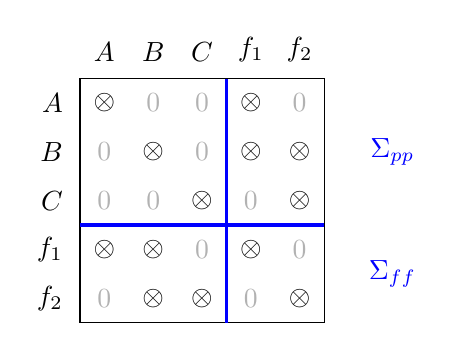
\begin{tikzpicture}[scale=0.62]
  % 5x5 grid of blocks: order A,B,C,f1,f2  (row 1 = top)
  \def\nz{{
    {1,0,0,1,0},
    {0,1,0,1,1},
    {0,0,1,0,1},
    {1,1,0,1,0},
    {0,1,1,0,1}}}
  \foreach \r in {0,...,4} {
    \foreach \c in {0,...,4} {
      \pgfmathparse{\nz[\r][\c]}
      \ifnum\pgfmathresult=1
        \node at (\c+0.5,4.5-\r) {$\otimes$};
      \else
        \node[gray!60] at (\c+0.5,4.5-\r) {$0$};
      \fi
    }
  }
  \draw (0,0) rectangle (5,5);
  % partition lines pose|feature at index 3
  \draw[blue,very thick] (3,0) -- (3,5);
  \draw[blue,very thick] (0,2) -- (5,2);
  % row / column labels
  \foreach \i/\nm in {0/A,1/B,2/C,3/f_1,4/f_2} {
    \node[left] at (-0.15,4.5-\i) {$\nm$};
    \node[above] at (\i+0.5,5.15) {$\nm$};
  }
  % block labels
  \node[blue] at (6.4,3.5) {$\vect{\Sigma}_{pp}$};
  \node[blue] at (6.4,1.0) {$\vect{\Sigma}_{ff}$};
\end{tikzpicture}
\caption{Sparsity of $\vect{\Sigma}=\vect{H}\trans\vect{H}$ ($\otimes$: nonzero block). The pose--pose block $\vect{\Sigma}_{pp}$ is block-diagonal, while $\vect{\Sigma}_{pf}$ records exactly which pose sees which feature. The information matrix reflects the problem structure.}
\label{fig:lec04-infomat}
\end{figure}

% =====================================================================
\subsection{A typical visual-odometry / SLAM pipeline}

How do the previous two lectures fit together into a working monocular system? A common pipeline incrementally grows poses $C_1,C_2,\dots$ and features $f_1,f_2,\dots$ (Fig.~\ref{fig:lec04-pipeline}):
\begin{enumerate}[label=(\arabic*),noitemsep,topsep=2pt]
\item \textbf{5-point algorithm} on $C_1,C_2$: recover ${}^{C_1}_{C_2}\vect{R}$ and ${}^{C_1}\vect{p}_{C_2}^{*}$ (up to scale).
\item \textbf{Feature triangulation}: with the recovered relative pose, triangulate $f_1,f_2,\dots$.
\item \textbf{P3P / PnP} for $C_3$: with known features, solve ${}^{C_1}_{C_3}\vect{R},\,{}^{C_1}\vect{p}_{C_3}$ (then triangulate new features).
\item \textbf{5-point or P3P/PnP} for $C_4$: solve ${}^{C_1}_{C_4}\vect{R},\,{}^{C_1}\vect{p}_{C_4}$.
\item \textbf{Bundle adjustment (BA)} over $C_1,C_2,C_3$ and $f_1,f_2,f_3,\dots$ (joint refinement of poses and structure).
\item \textbf{BA} extended to $C_1,C_2,C_3,C_4$ and $f_1,f_2,f_3,\dots$ as the window grows.
\item \textbf{Marginalization}: when there are too many poses ($C_1,\dots,C_n$) and features ($f_1,\dots,f_m$), marginalize old states $C_1,f_1,\dots$ to keep the system light-weight.
\end{enumerate}

\begin{figure}[H]
\centering
\begin{tikzpicture}[>=stealth,scale=1.0]
  % features (triangles) along the top
  \foreach \x/\nm in {2.0/f_1,3.0/f_2,4.0/f_3,6.3/f_4,7.6/f_5} {
    \node[draw,isosceles triangle,isosceles triangle apex angle=60,
          rotate=90,minimum size=5pt,inner sep=1pt,fill=black!10] at (\x,2.6) {};
    \node[above] at (\x,2.8) {\footnotesize $\nm$};
  }
  % camera frames along the bottom
  \foreach \x/\nm in {0.4/C_1,2.4/C_2,4.4/C_3,7.0/C_4} {
    \fill (\x,0) circle (1.6pt);
    \draw[->] (\x,0) -- (\x+0.4,0.16);
    \draw[->] (\x,0) -- (\x-0.1,0.40);
    \node[below] at (\x,-0.05) {\footnotesize $\nm$};
  }
  % a few observation rays (dashed, multi-color to suggest tracks)
  \draw[blue!70,dashed]   (0.4,0.15) -- (2.0,2.5);
  \draw[blue!70,dashed]   (0.4,0.15) -- (3.0,2.5);
  \draw[orange!80!black,dashed] (2.4,0.15) -- (2.0,2.5);
  \draw[orange!80!black,dashed] (2.4,0.15) -- (3.0,2.5);
  \draw[orange!80!black,dashed] (2.4,0.15) -- (4.0,2.5);
  \draw[green!55!black,dashed]  (4.4,0.15) -- (3.0,2.5);
  \draw[green!55!black,dashed]  (4.4,0.15) -- (4.0,2.5);
  \draw[green!55!black,dashed]  (4.4,0.15) -- (6.3,2.5);
  \draw[red!75!black,dashed]    (7.0,0.15) -- (6.3,2.5);
  \draw[red!75!black,dashed]    (7.0,0.15) -- (7.6,2.5);
\end{tikzpicture}
\caption{A monocular VO/SLAM pipeline grows poses $C_1,\dots,C_4$ and features $f_1,\dots,f_5$: bootstrap with the 5-point algorithm + triangulation, extend new poses with P3P/PnP, refine with bundle adjustment, and marginalize old states to bound cost. Combined with the previous two lectures, this builds up visual SLAM.}
\label{fig:lec04-pipeline}
\end{figure}

% =====================================================================
\subsection{Designing estimators: many ways to handle \texorpdfstring{$\vect{z}=\vect{h}(\vect{x})+\vect{n}$}{z=h(x)+n}}

Given $\vect{z} = \vect{h}(\vect{x}) + \vect{n}$, $\vect{n}\sim\mathcal{N}(\vect{0},\vect{R})$, there are many ways to linearize and solve, each leading to a different family of algorithms.

\paragraph{(1) Iterated re-linearization (GN / LM).} The typical solution $\min_{\vect{x}}\norm{\vect{z}-\vect{h}(\vect{x})}_{\vect{R}}^{2}$. Given a linearization $\hat{\vect{x}}$, $\tilde{\vect{z}} = \vect{H}\tilde{\vect{x}} + \vect{n}$; update $\vect{x}^{\oplus} = \hat{\vect{x}} + \tilde{\vect{x}}$, then \emph{redo} the linearization $\tilde{\vect{z}} = \vect{H}^{\oplus}\tilde{\vect{x}} + \vect{n}$ (Gauss--Newton or Levenberg--Marquardt).

\paragraph{(2) Linearize once + residual correction (FEJ).} What if we linearize only once, at a fixed $\hat{\vect{x}}^{0}$? With $\vect{H}^{0} = \vect{H}|_{\hat{\vect{x}}^{0}}$,
\begin{align}
\vect{z} &= \vect{h}(\hat{\vect{x}}^{0}) + \vect{H}^{0}(\vect{x}-\hat{\vect{x}}^{0}) + \vect{n} \\
\vect{z} - \vect{h}(\hat{\vect{x}}^{0}) &= \vect{H}^{0}\big(\vect{x} - \hat{\vect{x}} + \underbrace{\hat{\vect{x}} - \hat{\vect{x}}^{0}}_{\Delta\vect{x}}\big) + \vect{n}
= \vect{H}^{0}\tilde{\vect{x}} + \vect{H}^{0}\Delta\vect{x} + \vect{n},
\end{align}
so moving the known offset to the left gives the \emph{residual correction}
\begin{align}
\underbrace{\vect{z} - \vect{h}(\hat{\vect{x}}^{0})}_{\tilde{\vect{z}}^{0}} - \vect{H}^{0}\Delta\vect{x} = \vect{H}^{0}\tilde{\vect{x}} + \vect{n}.
\end{align}
Keeping the Jacobian fixed at the first estimate is \textbf{FEJ} (first-estimate Jacobians)~\cite{Huang2008ISER}, used e.g.\ in OKVIS~\cite{Leutenegger2014IJRR}; it preserves the correct observability/nullspace structure.

\paragraph{(3) Partial linearization (preintegration / iSAM).} For $\vect{x} = [\vect{x}_A\trans,\vect{x}_B\trans]\trans$, $\vect{z} = \vect{h}(\vect{x}_A,\vect{x}_B)+\vect{n}$, linearize only in $\vect{x}_B$ (about $\hat{\vect{x}}_B^{0}$) while keeping $\vect{x}_A$ exact:
\begin{align}
\vect{z} &= \vect{h}(\hat{\vect{x}}_A,\hat{\vect{x}}_B^{0}) + \vect{H}_A\tilde{\vect{x}}_A + \vect{H}_B^{0}\tilde{\vect{x}}_B + \vect{H}_B^{0}\Delta\vect{x}_B + \vect{n}, \\
\underbrace{\vect{z} - \vect{h}(\hat{\vect{x}}_A,\hat{\vect{x}}_B^{0})}_{\tilde{\vect{z}}^{0}} - \vect{H}_B^{0}\Delta\vect{x}_B
&= \begin{bmatrix} \vect{H}_A & \vect{H}_B^{0} \end{bmatrix}\begin{bmatrix} \tilde{\vect{x}}_A \\ \tilde{\vect{x}}_B \end{bmatrix} + \vect{n}.
\end{align}
This is the idea behind IMU \textbf{pre-integration}~\cite{Forster2017tro} and \textbf{ACI} (analytic combined integration)~\cite{Eckenhoff2017ICRA}; \textbf{iSAM}~\cite{Kaess2012IJRR} uses a similar partial-relinearization idea.

\paragraph{(4) Nullspace projection (MSCKF / structureless).} For $\vect{x}=[\vect{x}_A\trans,\vect{x}_B\trans]\trans$, $\tilde{\vect{z}} = \vect{H}_A\tilde{\vect{x}}_A + \vect{H}_B\tilde{\vect{x}}_B + \vect{n}$. If we find $\vect{N}$ with $\vect{N}\trans\vect{H}_B = \vect{0}$, then projecting onto the left nullspace removes $\vect{x}_B$:
\begin{align}
\vect{N}\trans\tilde{\vect{z}} = \vect{N}\trans\vect{H}_A\tilde{\vect{x}}_A + \cancel{\vect{N}\trans\vect{H}_B\tilde{\vect{x}}_B} + \vect{N}\trans\vect{n}.
\end{align}
This is the \textbf{MSCKF}~\cite{Mourikis2007ICRA} (multi-state constraint Kalman filter), a.k.a.\ the smart / structure-less vision factor: the features are eliminated without ever being added to the state.

\paragraph{(5) Invariant errors.} Instead of $\vect{x} = \hat{\vect{x}} + \tilde{\vect{x}}$, put $\vect{x}$ on a group $SE(3)$ / $SE_2(3)$ and use a right-invariant error,
\begin{align}
\vect{x} = \hat{\vect{x}}\boxplus\tilde{\vect{x}} = \Exp(\tilde{\vect{x}})\cdot\hat{\vect{x}} \;\Rightarrow\; \text{invariant SLAM / VIO}.
\end{align}

\paragraph{(6) Decoupled (right-)invariant errors.} For $\vect{x}=[\vect{x}_A\trans,\vect{x}_B\trans]\trans$, mix error types per block:
\begin{align}
\begin{cases}
\vect{x}_A = \hat{\vect{x}}_A\boxplus\tilde{\vect{x}}_A = \Exp(\tilde{\vect{x}}_A)\cdot\hat{\vect{x}}_A & \text{(group / invariant error)} \\
\vect{x}_B = \hat{\vect{x}}_B + \tilde{\vect{x}}_B & \text{(vector error)}
\end{cases}
\end{align}
which gives decoupled right-invariant SLAM / VIO.

\begin{quote}
Use your imagination to deal with $\big\{\vect{z}=\vect{h}(\vect{x})+\vect{n},\;\tilde{\vect{z}}=\vect{H}\tilde{\vect{x}}+\vect{n}\big\}$ to design different algorithms.
\end{quote}

% =====================================================================
\subsection{Designing a common system: from MAP to the EKF}

Consider the canonical prior + motion + measurement system
\begin{align}
\begin{cases}
\vect{x}_0 \sim \mathcal{N}(\hat{\vect{x}}_0,\vect{P}_0) & \to \text{prior} \\
\vect{x}_1 = \vect{f}(\vect{x}_0) + \vect{w}_0, \quad \vect{w}_k\sim\mathcal{N}(\vect{0},\vect{Q}) & \to \text{motion model} \\
\vect{z}_1 = \vect{h}(\vect{x}_1) + \vect{n}_1, \quad \vect{n}_1\sim\mathcal{N}(\vect{0},\vect{R}) & \to \text{measurement model}
\end{cases}
\end{align}
The MAP estimate factorizes by Bayes' rule,
\begin{align}
\max_{\vect{x}} p(\vect{x}\mid\vect{z})
= \max_{\vect{x}} \frac{p(\vect{z}\mid\vect{x})\,p(\vect{x})}{p(\vect{z})}
= \max_{\vect{x}} \frac{p(\vect{z}_1\mid\vect{x}_1)\,p(\vect{x}_1\mid\vect{x}_0)\,p(\vect{x}_0)}{p(\vect{z})},
\end{align}
which is equivalent to the nonlinear least-squares cost
\begin{align}
\min_{\vect{x}} \;\norm{\vect{z}_1 - \vect{h}(\vect{x}_1)}_{\vect{R}}^{2}
+ \norm{\vect{x}_1 - \vect{f}(\vect{x}_0)}_{\vect{Q}}^{2}
+ \norm{\vect{x}_0 - \hat{\vect{x}}_0}_{\vect{P}_0}^{2}.
\end{align}
There are two ways to solve it:
\begin{enumerate}[label=\arabic*.,noitemsep,topsep=2pt]
\item \textbf{Batch:} minimize all three terms jointly $\Rightarrow \hat{\vect{x}}_1,\vect{P}_1$.
\item \textbf{Incremental:}
  \begin{enumerate}[label=(\roman*),noitemsep,topsep=1pt]
  \item handle the prior + motion terms $\norm{\vect{x}_0-\hat{\vect{x}}_0}_{\vect{P}_0}^{2} + \norm{\vect{x}_1-\vect{f}(\vect{x}_0)}_{\vect{Q}}^{2}$;
  \item marginalize $\vect{x}_0$, keep $\vect{x}_1$, giving $(\hat{\vect{x}}_{1|0},\vect{P}_{1|0})$;
  \item add the measurement $\norm{\vect{x}_1-\hat{\vect{x}}_{1|0}}_{\vect{P}_{1|0}}^{2} + \norm{\vect{z}_1-\vect{h}(\vect{x}_1)}_{\vect{R}}^{2} \Rightarrow \hat{\vect{x}}_1,\vect{P}_1$.
  \end{enumerate}
\end{enumerate}
The incremental route is exactly the EKF predict/update, as we now derive.

\paragraph{Propagation (marginalize $\vect{x}_0$).} Linearize the motion model, $\vect{x}_1 = \vect{f}(\vect{x}_0)+\vect{w}_0 \Rightarrow \hat{\vect{x}}_1 + \tilde{\vect{x}}_1 = \vect{f}(\hat{\vect{x}}_0) + \vect{F}\tilde{\vect{x}}_0 + \vect{w}_0$, and define the motion residual
\begin{align}
\vect{r}_{\vect{x}} \triangleq \hat{\vect{x}}_1 - \vect{f}(\hat{\vect{x}}_0) = \vect{F}\tilde{\vect{x}}_0 - \tilde{\vect{x}}_1 + \vect{w}_0,
\qquad
\vect{w}_0 = \vect{r}_{\vect{x}} - \begin{bmatrix} \vect{F} & -\vect{I} \end{bmatrix}\begin{bmatrix} \tilde{\vect{x}}_0 \\ \tilde{\vect{x}}_1 \end{bmatrix}.
\end{align}
The prior + motion cost (writing $\vect{Q}_0=\vect{Q}$) is
\begin{align}
\min \; \norm{\tilde{\vect{x}}_0}_{\vect{P}_0}^{2}
+ \Big\|\,\vect{r}_{\vect{x}} - \begin{bmatrix} \vect{F} & -\vect{I} \end{bmatrix}\begin{bmatrix} \tilde{\vect{x}}_0 \\ \tilde{\vect{x}}_1 \end{bmatrix}\Big\|_{\vect{Q}_0}^{2}.
\end{align}
Collecting quadratic and linear terms, the cost $C$ is
\begin{align}
C = \begin{bmatrix} \tilde{\vect{x}}_0 \\ \tilde{\vect{x}}_1 \end{bmatrix}\trans
\begin{bmatrix} \vect{P}_0^{-1} + \vect{F}\trans\vect{Q}_0^{-1}\vect{F} & -\vect{F}\trans\vect{Q}_0^{-1} \\ -\vect{Q}_0^{-1}\vect{F} & \vect{Q}_0^{-1} \end{bmatrix}
\begin{bmatrix} \tilde{\vect{x}}_0 \\ \tilde{\vect{x}}_1 \end{bmatrix}
- 2\begin{bmatrix} \tilde{\vect{x}}_0 \\ \tilde{\vect{x}}_1 \end{bmatrix}\trans
\begin{bmatrix} \vect{F}\trans \\ -\vect{I} \end{bmatrix}\vect{Q}_0^{-1}\vect{r}_{\vect{x}}
+ \vect{r}_{\vect{x}}\trans\vect{Q}_0^{-1}\vect{r}_{\vect{x}}.
\end{align}
Setting $\partial C/\partial[\tilde{\vect{x}}_0;\tilde{\vect{x}}_1] = \vect{0}$ gives the information system
\begin{align}
\begin{bmatrix} \vect{P}_0^{-1} + \vect{F}\trans\vect{Q}_0^{-1}\vect{F} & -\vect{F}\trans\vect{Q}_0^{-1} \\ -\vect{Q}_0^{-1}\vect{F} & \vect{Q}_0^{-1} \end{bmatrix}
\begin{bmatrix} \tilde{\vect{x}}_0 \\ \tilde{\vect{x}}_1 \end{bmatrix}
= \begin{bmatrix} \vect{F}\trans\vect{Q}_0^{-1}\vect{r}_{\vect{x}} \\ -\vect{Q}_0^{-1}\vect{r}_{\vect{x}} \end{bmatrix}.
\end{align}
Marginalizing $\vect{x}_0$ (Schur complement onto the $\vect{x}_1$ block) and applying the matrix inversion lemma,
\begin{align}
\Big[\vect{Q}_0^{-1} - \vect{Q}_0^{-1}\vect{F}\big(\vect{P}_0^{-1} + \vect{F}\trans\vect{Q}_0^{-1}\vect{F}\big)^{-1}\vect{F}\trans\vect{Q}_0^{-1}\Big]\tilde{\vect{x}}_1
&= -\vect{Q}_0^{-1}\vect{r}_{\vect{x}} + \vect{Q}_0^{-1}\vect{F}\big(\vect{P}_0^{-1}+\vect{F}\trans\vect{Q}_0^{-1}\vect{F}\big)^{-1}\vect{F}\trans\vect{Q}_0^{-1}\vect{r}_{\vect{x}}, \notag \\
\underbrace{\big(\vect{Q}_0 + \vect{F}\vect{P}_0\vect{F}\trans\big)^{-1}}_{\vect{P}_{1|0}^{-1}}\tilde{\vect{x}}_1
&= -\big(\vect{Q}_0 + \vect{F}\vect{P}_0\vect{F}\trans\big)^{-1}\vect{r}_{\vect{x}}.
\end{align}
This is the EKF \textbf{propagation}: the predicted covariance and mean are
\begin{empheq}[box=\fbox]{align}
\vect{P}_{1|0} = \vect{F}\vect{P}_0\vect{F}\trans + \vect{Q}_0, \qquad
\hat{\vect{x}}_{1|0} = \vect{f}(\hat{\vect{x}}_0) \;\;(\text{i.e.\ }\vect{r}_{\vect{x}}=\vect{0}).
\end{empheq}

\paragraph{Update (add the measurement).} Now include the measurement $\vect{z}_1 = \vect{h}(\vect{x}_1)+\vect{n}\Rightarrow\tilde{\vect{z}}=\vect{H}\tilde{\vect{x}}_1+\vect{n}$. The full cost
\begin{align}
\norm{\tilde{\vect{z}} - \vect{H}\tilde{\vect{x}}_1}_{\vect{R}}^{2}
+ \Big\|\vect{r}_{\vect{x}} - \begin{bmatrix}\vect{F} & -\vect{I}\end{bmatrix}\begin{bmatrix}\tilde{\vect{x}}_0\\\tilde{\vect{x}}_1\end{bmatrix}\Big\|_{\vect{Q}_0}^{2}
+ \norm{\tilde{\vect{x}}_0}_{\vect{P}_0}^{2}
\end{align}
yields the augmented information system (the measurement adds $\vect{H}\trans\vect{R}^{-1}\vect{H}$ to the $\vect{x}_1$ block and $\vect{H}\trans\vect{R}^{-1}\tilde{\vect{z}}$ to its residual),
\begin{align}
\begin{bmatrix} \vect{P}_0^{-1} + \vect{F}\trans\vect{Q}_0^{-1}\vect{F} & -\vect{F}\trans\vect{Q}_0^{-1} \\ -\vect{Q}_0^{-1}\vect{F} & \vect{Q}_0^{-1} + \vect{H}\trans\vect{R}^{-1}\vect{H} \end{bmatrix}
\begin{bmatrix} \tilde{\vect{x}}_0 \\ \tilde{\vect{x}}_1 \end{bmatrix}
= \begin{bmatrix} \vect{F}\trans\vect{Q}_0^{-1}\vect{r}_{\vect{x}} \\ -\vect{Q}_0^{-1}\vect{r}_{\vect{x}} + \vect{H}\trans\vect{R}^{-1}\tilde{\vect{z}} \end{bmatrix}.
\end{align}
Marginalizing $\vect{x}_0$ again and recognizing $\vect{P}_{1|0}^{-1} = (\vect{Q}_0+\vect{F}\vect{P}_0\vect{F}\trans)^{-1}$,
\begin{align}
\underbrace{\big(\vect{H}\trans\vect{R}^{-1}\vect{H} + \vect{P}_{1|0}^{-1}\big)}_{\vect{\Sigma}\,=\,\vect{P}_{1|1}^{-1}}\tilde{\vect{x}}_1
= \vect{H}\trans\vect{R}^{-1}\tilde{\vect{z}} - \underbrace{\vect{P}_{1|0}^{-1}\vect{r}_{\vect{x}}}_{\to\,\vect{0}}.
\end{align}
After propagation $\vect{r}_{\vect{x}}=\vect{0}$, so the second term drops. Applying the matrix inversion lemma to the updated covariance,
\begin{align}
\vect{P}_{1|1} = \big(\vect{P}_{1|0}^{-1} + \vect{H}\trans\vect{R}^{-1}\vect{H}\big)^{-1}
= \vect{P}_{1|0} - \vect{P}_{1|0}\vect{H}\trans\big(\vect{H}\vect{P}_{1|0}\vect{H}\trans + \vect{R}\big)^{-1}\vect{H}\vect{P}_{1|0},
\end{align}
and for the mean correction, using the same lemma to convert information $\to$ covariance form,
\begin{align}
\tilde{\vect{x}}_1
&= \big(\vect{P}_{1|0}^{-1} + \vect{H}\trans\vect{R}^{-1}\vect{H}\big)^{-1}\vect{H}\trans\vect{R}^{-1}\tilde{\vect{z}} \\
&= \Big(\vect{P}_{1|0} - \vect{P}_{1|0}\vect{H}\trans\big(\vect{H}\vect{P}_{1|0}\vect{H}\trans+\vect{R}\big)^{-1}\vect{H}\vect{P}_{1|0}\Big)\vect{H}\trans\vect{R}^{-1}\tilde{\vect{z}} \\
&= \vect{P}_{1|0}\vect{H}\trans\Big(\vect{R}^{-1} - \big(\vect{H}\vect{P}_{1|0}\vect{H}\trans+\vect{R}\big)^{-1}\vect{H}\vect{P}_{1|0}\vect{H}\trans\vect{R}^{-1}\Big)\tilde{\vect{z}} \\
&= \vect{P}_{1|0}\vect{H}\trans\big(\vect{H}\vect{P}_{1|0}\vect{H}\trans+\vect{R}\big)^{-1}\Big(\big(\vect{H}\vect{P}_{1|0}\vect{H}\trans+\vect{R}\big)\vect{R}^{-1} - \vect{H}\vect{P}_{1|0}\vect{H}\trans\vect{R}^{-1}\Big)\tilde{\vect{z}} \\
&= \vect{P}_{1|0}\vect{H}\trans\big(\vect{H}\vect{P}_{1|0}\vect{H}\trans+\vect{R}\big)^{-1}\tilde{\vect{z}}.
\end{align}
Finally, with the Kalman gain $\vect{K} = \vect{P}_{1|0}\vect{H}\trans(\vect{H}\vect{P}_{1|0}\vect{H}\trans+\vect{R})^{-1}$, we recover the EKF \textbf{update}:
\begin{empheq}[box=\fbox]{align}
\tilde{\vect{x}}_1 = \vect{P}_{1|0}\vect{H}\trans\big(\vect{H}\vect{P}_{1|0}\vect{H}\trans+\vect{R}\big)^{-1}\tilde{\vect{z}}, \qquad
\vect{P}_{1|1} = \vect{P}_{1|0} - \vect{P}_{1|0}\vect{H}\trans\big(\vect{H}\vect{P}_{1|0}\vect{H}\trans+\vect{R}\big)^{-1}\vect{H}\vect{P}_{1|0}.
\end{empheq}
The extended Kalman filter is thus the incremental (marginalize-then-update) solution of the same MAP problem that batch least squares solves jointly --- the two views are connected by the matrix inversion lemma and the Schur complement.

% =====================================================================
\subsection{The relationship between Schur complement and nullspace projection}

The Schur-complement marginalization (\S4.3) and the nullspace projection (\S4.6, item~4, the MSCKF) both eliminate $\vect{x}_B$ --- it turns out they are the \emph{same} operation. Take $\vect{z} = \vect{h}(\vect{x}_A,\vect{x}_B) + \vect{n}$, $\vect{n}\sim\mathcal{N}(\vect{0},\vect{R})$, with $\tilde{\vect{z}} = \vect{H}_A\tilde{\vect{x}}_A + \vect{H}_B\tilde{\vect{x}}_B + \vect{n}$.

\paragraph{(1) Information form.} The normal equations are
\begin{align}
\begin{bmatrix} \vect{H}_A\trans\vect{R}^{-1}\vect{H}_A & \vect{H}_A\trans\vect{R}^{-1}\vect{H}_B \\ \vect{H}_B\trans\vect{R}^{-1}\vect{H}_A & \vect{H}_B\trans\vect{R}^{-1}\vect{H}_B \end{bmatrix}
\begin{bmatrix} \tilde{\vect{x}}_A \\ \tilde{\vect{x}}_B \end{bmatrix}
= \begin{bmatrix} \vect{H}_A\trans \\ \vect{H}_B\trans \end{bmatrix}\vect{R}^{-1}\tilde{\vect{z}}.
\end{align}
Marginalizing $\vect{x}_B$ and keeping $\vect{x}_A$ via the Schur complement gives
\begin{empheq}[box=\fbox]{align}
\underbrace{\big(\vect{H}_A\trans\vect{R}^{-1}\vect{H}_A - \vect{H}_A\trans\vect{R}^{-1}\vect{H}_B(\vect{H}_B\trans\vect{R}^{-1}\vect{H}_B)^{-1}\vect{H}_B\trans\vect{R}^{-1}\vect{H}_A\big)}_{\text{information}}\tilde{\vect{x}}_A & \notag\\
= \underbrace{\vect{H}_A\trans\vect{R}^{-1}\tilde{\vect{z}} - \vect{H}_A\trans\vect{R}^{-1}\vect{H}_B(\vect{H}_B\trans\vect{R}^{-1}\vect{H}_B)^{-1}\vect{H}_B\trans\vect{R}^{-1}\tilde{\vect{z}}}_{\text{residual}}&. \tag{Eq.\ 1}
\end{empheq}

\paragraph{(2) Nullspace form.} Take a (thin) QR-type factorization of $\vect{H}_B$,
\begin{align}
\vect{H}_B = \begin{bmatrix} \vect{Q}_e & \vect{Q}_N \end{bmatrix}\begin{bmatrix} \vect{U} \\ \vect{0} \end{bmatrix} = \vect{Q}_e\vect{U} + \vect{Q}_N\cdot\vect{0} = \vect{Q}_e\vect{U},
\end{align}
with $\vect{U}$ upper triangular and $[\vect{Q}_e\;\vect{Q}_N]$ orthogonal, so $\vect{Q}_e\vect{Q}_e\trans + \vect{Q}_N\vect{Q}_N\trans = \vect{I}$, $\vect{Q}_e\trans\vect{Q}_e = \vect{I}$, $\vect{Q}_N\trans\vect{Q}_N = \vect{I}$, and the left nullspace satisfies $\vect{Q}_N\trans\vect{H}_B = \vect{Q}_N\trans\vect{Q}_e\vect{U} = \vect{0}$. Projecting the residual onto $\vect{Q}_N$ removes $\vect{x}_B$:
\begin{align}
\vect{Q}_N\trans\tilde{\vect{z}} = \vect{Q}_N\trans\vect{H}_A\tilde{\vect{x}}_A + \cancel{\vect{Q}_N\trans\vect{H}_B\tilde{\vect{x}}_B} + \vect{Q}_N\trans\vect{n}
= \vect{Q}_N\trans\vect{H}_A\tilde{\vect{x}}_A + \vect{Q}_N\trans\vect{n},
\end{align}
with projected noise covariance $\vect{Q}_N\trans\vect{R}\vect{Q}_N$. The resulting normal equations are
\begin{empheq}[box=\fbox]{align}
(\vect{Q}_N\trans\vect{H}_A)\trans(\vect{Q}_N\trans\vect{R}\vect{Q}_N)^{-1}(\vect{Q}_N\trans\vect{H}_A)\,\tilde{\vect{x}}_A
= (\vect{Q}_N\trans\vect{H}_A)\trans(\vect{Q}_N\trans\vect{R}\vect{Q}_N)^{-1}\vect{Q}_N\trans\tilde{\vect{z}}. \tag{Eq.\ 2}
\end{empheq}

\paragraph{Are Eq.~1 and Eq.~2 equivalent?} Consider the isotropic case $\vect{R} = \sigma^2\vect{I}$. With $\vect{H}_B = \vect{Q}_e\vect{U}$,
\begin{align}
\vect{H}_B\trans\vect{R}^{-1}\vect{H}_B = (\vect{Q}_e\vect{U})\trans\frac{\vect{I}}{\sigma^2}\vect{Q}_e\vect{U} = \frac{\vect{U}\trans\vect{U}}{\sigma^2},
\end{align}
so the projector that appears in the Schur complement of Eq.~1 is
\begin{align}
\vect{H}_A\trans\vect{R}^{-1}\vect{H}_B(\vect{H}_B\trans\vect{R}^{-1}\vect{H}_B)^{-1}\vect{H}_B\trans\vect{R}^{-1}\vect{H}_A
&= \vect{H}_A\trans\frac{\vect{I}}{\sigma^2}\vect{Q}_e\vect{U}\,\sigma^2(\vect{U}\trans\vect{U})^{-1}\vect{U}\trans\vect{Q}_e\trans\frac{\vect{I}}{\sigma^2}\vect{H}_A \notag\\
&= \frac{1}{\sigma^2}\vect{H}_A\trans\vect{Q}_e\vect{Q}_e\trans\vect{H}_A.
\end{align}
Hence the Eq.~1 information becomes, using $\vect{Q}_e\vect{Q}_e\trans = \vect{I} - \vect{Q}_N\vect{Q}_N\trans$,
\begin{align}
\frac{1}{\sigma^2}\vect{H}_A\trans\vect{H}_A - \frac{1}{\sigma^2}\vect{H}_A\trans\vect{Q}_e\vect{Q}_e\trans\vect{H}_A
= \frac{1}{\sigma^2}\vect{H}_A\trans\big(\vect{I} - \vect{Q}_e\vect{Q}_e\trans\big)\vect{H}_A
= \frac{1}{\sigma^2}\vect{H}_A\trans\vect{Q}_N\vect{Q}_N\trans\vect{H}_A.
\end{align}
The Eq.~2 information, using $\vect{Q}_N\trans\vect{R}\vect{Q}_N = \sigma^2\vect{Q}_N\trans\vect{Q}_N = \sigma^2\vect{I}$, is
\begin{align}
(\vect{Q}_N\trans\vect{H}_A)\trans(\sigma^2\vect{I})^{-1}(\vect{Q}_N\trans\vect{H}_A) = \frac{1}{\sigma^2}\vect{H}_A\trans\vect{Q}_N\vect{Q}_N\trans\vect{H}_A,
\end{align}
which is identical (the residuals match the same way). Therefore, for isotropic noise, Schur-complement marginalization and left-nullspace projection produce exactly the same information and residual --- the MSCKF's structureless update is precisely the marginalization of the feature.
